\documentclass[12pt]{article}
\usepackage{fancyhdr}
\usepackage{amsmath,amsfonts,enumerate}
\usepackage{color,graphicx}
\usepackage{tikz}
\usepackage{pgfplots}
\usepackage{listings}
\usepackage{algorithm}
\usepackage{algorithmic}
\usetikzlibrary{arrows,positioning,shapes,calc,matrix}
\pagestyle{fancy}

% Define colors for answers
\definecolor{answercolor}{RGB}{0,100,0}
\definecolor{explanationcolor}{RGB}{0,0,139}

% Custom commands for answers
\newcommand{\answer}[1]{{\color{answercolor}\textbf{Answer:} #1}}
\newcommand{\explanation}[1]{{\color{explanationcolor}#1}}

%%%%%%%%%%%%%%%%%%%%%%%%%%%%%%%%%%%%%%%%%%%%%%%%%
% Course customization based on Professor's teaching
%%%%%%%%%%%%%%%%%%%%%%%%%%%%%%%%%%%%%%%%%%%%%%%%%
\newcommand{\masunitnumber}{CENG 403}
\newcommand{\examdate}{January 2025}
\newcommand{\academicyear}{2024-2025}
\newcommand{\semester}{I}
\newcommand{\coursename}{Deep Learning - RNNs, Language Modeling \& Word Embeddings - ANSWERED}
\newcommand{\numberofhours}{3}
%%%%%%%%%%%%%%%%%%%%%%%%%%%%%%%%%%%%%%%%%%%%%%%%%
% CUSTOM SPACING COMMANDS FOR ANSWER SPACES
%%%%%%%%%%%%%%%%%%%%%%%%%%%%%%%%%%%%%%%%%%%%%%%%%
\newcommand{\answerspace}[1]{\vspace{#1}}
\newcommand{\questionspace}{\vspace{3cm}}        
\newcommand{\subquestionspace}{\vspace{2.5cm}}   
\newcommand{\shortanswer}{\vspace{2cm}}          
\newcommand{\mediumanswer}{\vspace{3cm}}         
\newcommand{\longanswer}{\vspace{4cm}}           
\newcommand{\journalspace}{\vspace{4.5cm}}       
\newcommand{\codespace}{\vspace{5cm}}            
%%%%%%%%%%%%%%%%%%%%%%%%%%%%%%%%%%%%%%%%%%%%%%%%%
% Header setup
%%%%%%%%%%%%%%%%%%%%%%%%%%%%%%%%%%%%%%%%%%%%%%%%%
\lhead{}
\rhead{}
\chead{{\bf MIDDLE EAST TECHNICAL UNIVERSITY}}
\lfoot{}
\rfoot{}
\cfoot{}
\begin{document}
\setlength{\headsep}{5truemm}
\setlength{\headheight}{14.5truemm}
\setlength{\voffset}{-0.45truein}
\renewcommand{\headrulewidth}{0.0pt}
\begin{center}
SEMESTER \semester\ EXAMINATION \academicyear
\end{center}
\begin{center}
{\bf \masunitnumber\ -- \coursename}
\end{center}
\vspace{20truemm}
\noindent \examdate\hspace{45truemm} TIME ALLOWED: \numberofhours\ HOURS
\vspace{19truemm}
\hrule
\vspace{19truemm}
\noindent\underline{INSTRUCTIONS TO CANDIDATES}
\vspace{8truemm}
%%%%%%%%%%%%%%%%%%%%%%%%%%%%%%%%%%%%%%%%%%%%%%%%%%%%%%
% Instructions based on professor's emphasis
%%%%%%%%%%%%%%%%%%%%%%%%%%%%%%%%%%%%%%%%%%%%%%%%%%%%%%
\begin{enumerate}
\item This examination paper contains {\bf SIX (6)} questions and comprises 
{\bf EIGHT (8)} printed pages.
\item Answer all questions. 
The marks for each question are indicated at the beginning of each question.
\item Answer each question beginning on a {\bf FRESH} page of the answer book.
\item This {\bf IS NOT an OPEN BOOK} exam.
\item Show clear reasoning for your answers, especially intuitive explanations.
\item For algorithms, provide step-by-step explanations as taught in lectures.
\item Draw diagrams where requested and explain information flow clearly.
\item Connect concepts to modern applications (LLMs, etc.) where relevant.
\end{enumerate}
%%%%%%%%%%%%%%%%%%%%%%%%%%%%%%%%%%%%%%%%%%%%%%%%%
% New page for questions
%%%%%%%%%%%%%%%%%%%%%%%%%%%%%%%%%%%%%%%%%%%%%%%%%
\newpage
\lhead{}
\rhead{\masunitnumber}
\chead{}
\lfoot{}
\cfoot{\thepage}
\rfoot{}
\setlength{\footskip}{45pt}
%%%%%%%%%%%%%%%%%%%%%%%%%%%%%%%%%%%%%%%%%%%%%%%%%%
% EXAM QUESTIONS BASED ON PROFESSOR'S TEACHING
%%%%%%%%%%%%%%%%%%%%%%%%%%%%%%%%%%%%%%%%%%%%%%%%%%

\paragraph{Question 1. RNN Backpropagation and Weight Sharing}\hfill (25 marks)\\
Based on the professor's explanation of how RNNs work as "feedforward networks with weight sharing across time."

\begin{enumerate}[(a)]
    \item The professor emphasized that "we need to be careful about weight sharing when calculating gradients." Explain why we must sum gradients from all time steps for a single weight parameter in an RNN. Use a concrete example with 3 time steps. \hfill (8 marks)
    
    \answer{We must sum gradients because the same weight appears at multiple time steps in the unfolded network, and each appearance contributes to the final loss through different paths.}
    
    \explanation{
    \textbf{Weight Sharing in RNNs:}
    
    \textbf{Fundamental Principle:}
    \begin{itemize}
        \item RNN uses the same weight matrix $W_{hh}$ at every time step
        \item When unfolded, this creates multiple "copies" of the same weight
        \item Each copy contributes to the loss through different computational paths
        \item Total gradient = sum of gradients from all copies
    \end{itemize}
    
    \textbf{Concrete Example with 3 Time Steps:}
    
    Consider RNN: $h_t = \tanh(W_{hh} h_{t-1} + W_{hx} x_t + b)$
    
    \textbf{Unfolded equations:}
    \begin{align}
    h_1 &= \tanh(W_{hh} h_0 + W_{hx} x_1 + b) \\
    h_2 &= \tanh(W_{hh} h_1 + W_{hx} x_2 + b) \\
    h_3 &= \tanh(W_{hh} h_2 + W_{hx} x_3 + b)
    \end{align}
    
    \textbf{Gradient Contributions for $W_{hh}$:}
    
    The weight $W_{hh}$ appears in three different contexts:
    \begin{itemize}
        \item \textbf{At $t=1$:} Directly affects $h_1$, which influences $h_2$ and $h_3$
        \item \textbf{At $t=2$:} Directly affects $h_2$, which influences $h_3$
        \item \textbf{At $t=3$:} Directly affects $h_3$
    \end{itemize}
    
    \textbf{Mathematical Gradient Computation:}
    $$\frac{\partial L}{\partial W_{hh}} = \frac{\partial L}{\partial h_1} \frac{\partial h_1}{\partial W_{hh}} + \frac{\partial L}{\partial h_2} \frac{\partial h_2}{\partial W_{hh}} + \frac{\partial L}{\partial h_3} \frac{\partial h_3}{\partial W_{hh}}$$
    
    Where:
    \begin{itemize}
        \item $\frac{\partial h_1}{\partial W_{hh}} = h_0 \cdot (1 - h_1^2)$ (direct contribution)
        \item $\frac{\partial h_2}{\partial W_{hh}} = h_1 \cdot (1 - h_2^2)$ (direct contribution)
        \item $\frac{\partial h_3}{\partial W_{hh}} = h_2 \cdot (1 - h_3^2)$ (direct contribution)
    \end{itemize}
    
    \textbf{Why Summing is Essential:}
    \begin{itemize}
        \item Each time step provides learning signal about optimal $W_{hh}$ value
        \item Ignoring any contribution loses information about how $W_{hh}$ should change
        \item Professor's emphasis on "careful" refers to ensuring no gradient contributions are missed
        \item This is fundamental difference from feedforward networks where each weight appears only once
    \end{itemize}
    }
    
    \item During backpropagation through time, the professor stressed that "we need to start from the end because earlier copies contribute to all following time steps." Draw and explain the gradient flow through an unfolded RNN showing why this order is essential. \hfill (10 marks)
    
    \begin{center}
    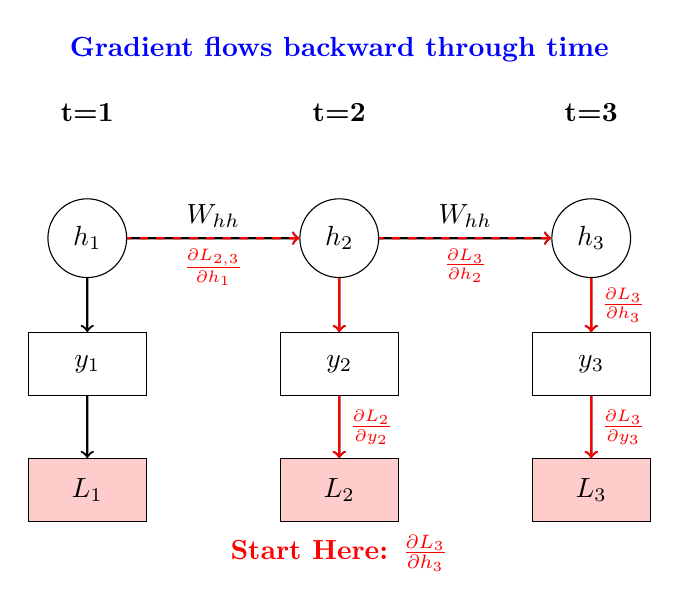
\begin{tikzpicture}[scale=0.8]
        % Time steps
        \node at (2,7) {\textbf{t=1}};
        \node at (6,7) {\textbf{t=2}};
        \node at (10,7) {\textbf{t=3}};
        
        % Hidden states
        \node[draw, circle, minimum size=1cm] (h1) at (2,5) {$h_1$};
        \node[draw, circle, minimum size=1cm] (h2) at (6,5) {$h_2$};
        \node[draw, circle, minimum size=1cm] (h3) at (10,5) {$h_3$};
        
        % Outputs
        \node[draw, rectangle, minimum width=1.5cm, minimum height=0.8cm] (y1) at (2,3) {$y_1$};
        \node[draw, rectangle, minimum width=1.5cm, minimum height=0.8cm] (y2) at (6,3) {$y_2$};
        \node[draw, rectangle, minimum width=1.5cm, minimum height=0.8cm] (y3) at (10,3) {$y_3$};
        
        % Losses
        \node[draw, rectangle, minimum width=1.5cm, minimum height=0.8cm, fill=red!20] (L1) at (2,1) {$L_1$};
        \node[draw, rectangle, minimum width=1.5cm, minimum height=0.8cm, fill=red!20] (L2) at (6,1) {$L_2$};
        \node[draw, rectangle, minimum width=1.5cm, minimum height=0.8cm, fill=red!20] (L3) at (10,1) {$L_3$};
        
        % Forward connections
        \draw[thick, ->] (h1) -- (h2) node[midway, above] {$W_{hh}$};
        \draw[thick, ->] (h2) -- (h3) node[midway, above] {$W_{hh}$};
        \draw[thick, ->] (h1) -- (y1);
        \draw[thick, ->] (h2) -- (y2);
        \draw[thick, ->] (h3) -- (y3);
        \draw[thick, ->] (y1) -- (L1);
        \draw[thick, ->] (y2) -- (L2);
        \draw[thick, ->] (y3) -- (L3);
        
        % Backward gradient flow
        \draw[thick, red, <-] (L3) -- (y3) node[midway, right, red] {\small $\frac{\partial L_3}{\partial y_3}$};
        \draw[thick, red, <-] (y3) -- (h3) node[midway, right, red] {\small $\frac{\partial L_3}{\partial h_3}$};
        
        \draw[thick, red, <-] (L2) -- (y2) node[midway, right, red] {\small $\frac{\partial L_2}{\partial y_2}$};
        \draw[thick, red, <-] (y2) -- (h2);
        
        % Critical backward connections
        \draw[thick, red, <-, dashed] (h3) -- (h2) node[midway, below, red] {\small $\frac{\partial L_3}{\partial h_2}$};
        \draw[thick, red, <-, dashed] (h2) -- (h1) node[midway, below, red] {\small $\frac{\partial L_{2,3}}{\partial h_1}$};
        
        % Labels
        \node[red] at (6,0) {\textbf{Start Here: $\frac{\partial L_3}{\partial h_3}$}};
        \node[blue] at (6,8) {\textbf{Gradient flows backward through time}};
    \end{tikzpicture}
    \end{center}
    
    \explanation{
    \textbf{Why Start from the End:}
    
    \textbf{Dependency Chain:}
    \begin{itemize}
        \item $h_3$ depends on $h_2$, which depends on $h_1$
        \item To compute $\frac{\partial L}{\partial h_2}$, we need $\frac{\partial L}{\partial h_3}$ (from future time step)
        \item To compute $\frac{\partial L}{\partial h_1}$, we need both $\frac{\partial L}{\partial h_2}$ and $\frac{\partial L}{\partial h_3}$
    \end{itemize}
    
    \textbf{Mathematical Justification:}
    
    \textbf{Gradient at $h_2$:}
    $$\frac{\partial L}{\partial h_2} = \frac{\partial L_2}{\partial h_2} + \frac{\partial L_3}{\partial h_2}$$
    
    The second term requires: $\frac{\partial L_3}{\partial h_2} = \frac{\partial L_3}{\partial h_3} \frac{\partial h_3}{\partial h_2}$
    
    \textbf{Gradient at $h_1$:}
    $$\frac{\partial L}{\partial h_1} = \frac{\partial L_1}{\partial h_1} + \frac{\partial L_2}{\partial h_1} + \frac{\partial L_3}{\partial h_1}$$
    
    Where:
    \begin{itemize}
        \item $\frac{\partial L_2}{\partial h_1} = \frac{\partial L_2}{\partial h_2} \frac{\partial h_2}{\partial h_1}$ (requires $\frac{\partial L_2}{\partial h_2}$)
        \item $\frac{\partial L_3}{\partial h_1} = \frac{\partial L_3}{\partial h_3} \frac{\partial h_3}{\partial h_2} \frac{\partial h_2}{\partial h_1}$ (requires both future gradients)
    \end{itemize}
    
    \textbf{Algorithm Order (Backpropagation Through Time):}
    \begin{enumerate}
        \item \textbf{Step 1:} Compute $\frac{\partial L_3}{\partial h_3}$ (direct from loss)
        \item \textbf{Step 2:} Compute $\frac{\partial L}{\partial h_2} = \frac{\partial L_2}{\partial h_2} + \frac{\partial L_3}{\partial h_3} \frac{\partial h_3}{\partial h_2}$
        \item \textbf{Step 3:} Compute $\frac{\partial L}{\partial h_1}$ using all future gradients
        \item \textbf{Step 4:} Sum gradients for shared weights across all time steps
    \end{enumerate}
    
    \textbf{Professor's Key Insight:}
    \begin{itemize}
        \item "Earlier copies contribute to all following time steps" means $h_1$ affects losses $L_1, L_2, L_3$
        \item Cannot compute total gradient for $h_1$ without knowing future contributions
        \item This creates strict dependency order: future → present → past
        \item Essential for correct gradient computation in weight sharing scenario
    \end{itemize}
    }
    
    \item The professor mentioned that RNNs suffer from "exploding gradient problem if weight norms are large, vanishing gradient problem if norms are small." Explain the mathematical reasoning behind both problems and why LSTM addresses these issues. \hfill (7 marks)
    
    \answer{Both problems stem from multiplicative gradient flow through recurrent connections. Large weights cause exponential growth, small weights cause exponential decay. LSTM uses additive cell state updates to avoid multiplicative accumulation.}
    
    \explanation{
    \textbf{Mathematical Analysis of Gradient Problems:}
    
    \textbf{Gradient Flow in RNN:}
    For $h_t = \tanh(W_{hh} h_{t-1} + W_{hx} x_t + b)$
    
    $$\frac{\partial h_t}{\partial h_{t-1}} = W_{hh} \cdot \text{diag}(\tanh'(u_t))$$
    
    \textbf{Long-term Gradient:}
    $$\frac{\partial h_T}{\partial h_1} = \prod_{t=2}^T W_{hh} \cdot \text{diag}(\tanh'(u_t))$$
    
    \textbf{Exploding Gradients (Large Weight Norms):}
    
    \textbf{Condition:} $\|W_{hh}\| > 1$ (spectral radius > 1)
    
    \textbf{Mathematical Reasoning:}
    \begin{itemize}
        \item Product of matrices with norm > 1 grows exponentially
        \item Even with $\tanh'(\cdot) \leq 1$, if $\|W_{hh}\| \gg 1$, product explodes
        \item Gradient magnitude: $\left\|\frac{\partial h_T}{\partial h_1}\right\| \approx \|W_{hh}\|^{T-1}$
        \item Example: $\|W_{hh}\| = 2$, $T = 50 \Rightarrow$ magnitude $\approx 2^{49} \approx 5 \times 10^{14}$
    \end{itemize}
    
    \textbf{Consequences:}
    \begin{itemize}
        \item Gradient updates become enormous
        \item Weights change drastically, causing instability
        \item Loss oscillates or diverges
        \item Training becomes impossible
    \end{itemize}
    
    \textbf{Vanishing Gradients (Small Weight Norms):}
    
    \textbf{Condition:} $\|W_{hh}\| < 1$ and/or small $\tanh'$ values
    
    \textbf{Mathematical Reasoning:}
    \begin{itemize}
        \item Product of matrices with norm < 1 decays exponentially
        \item $\tanh'(x) \in (0,1]$, typically much smaller than 1 for saturated neurons
        \item Combined effect: $\left\|\frac{\partial h_T}{\partial h_1}\right\| \approx \|W_{hh}\|^{T-1} \prod_{t=2}^T \|\tanh'(u_t)\|$
        \item Example: $\|W_{hh}\| = 0.5$, $\|\tanh'(u_t)\| = 0.3 \Rightarrow$ magnitude $\approx (0.5 \times 0.3)^{49} \approx 10^{-35}$
    \end{itemize}
    
    \textbf{Consequences:}
    \begin{itemize}
        \item Early time steps receive negligible gradients
        \item Cannot learn long-term dependencies
        \item Training focuses only on short-term patterns
        \item Information from distant past is effectively ignored
    \end{itemize}
    
    \textbf{How LSTM Addresses These Issues:}
    
    \textbf{Key Innovation: Additive Cell State Updates}
    $$C_t = f_t \odot C_{t-1} + i_t \odot \tilde{C}_t$$
    
    \textbf{Gradient Flow Through Cell State:}
    $$\frac{\partial C_t}{\partial C_{t-1}} = f_t$$
    
    \textbf{Advantages:}
    \begin{itemize}
        \item \textbf{No Weight Matrix Multiplication:} Gradient doesn't depend on $W_{hh}$
        \item \textbf{Learnable Control:} $f_t$ is learned, can be set to preserve gradients
        \item \textbf{Additive Nature:} $C_t = f_t \odot C_{t-1} + (\text{new info})$ avoids multiplicative accumulation
        \item \textbf{Gradient Preservation:} If $f_t \approx 1$, then $\frac{\partial C_T}{\partial C_1} \approx 1$
    \end{itemize}
    
    \textbf{Long-term LSTM Gradient:}
    $$\frac{\partial C_T}{\partial C_1} = \prod_{t=2}^T f_t$$
    
    \textbf{Why This Solves the Problems:}
    \begin{itemize}
        \item \textbf{Exploding:} $f_t \in [0,1]$ (sigmoid output) prevents explosion
        \item \textbf{Vanishing:} Network can learn $f_t \approx 1$ when long-term memory needed
        \item \textbf{Selective:} Can choose when to remember ($f_t \approx 1$) vs. forget ($f_t \approx 0$)
        \item \textbf{Stable:} Provides consistent gradient highway for learning
    \end{itemize}
    }
\end{enumerate}

\newpage
\paragraph{Question 2. Autoregressive Language Modeling}\hfill (20 marks)\\
The professor stated: "This is how large language models are trained as well - just to predict the next character."

\begin{enumerate}[(a)]
    \item Define autoregressive modeling as explained by the professor. Write the mathematical formulation for modeling $P(x_t | x_{t-1}, x_{t-2}, \ldots, x_1)$ and explain why this is considered "self-supervised learning." \hfill (8 marks)
    
    \answer{Autoregressive modeling predicts each token based on all previous tokens in sequence. It's self-supervised because the training data provides both inputs and targets from the same sequence without external labels.}
    
    \explanation{
    \textbf{Definition of Autoregressive Modeling:}
    
    \textbf{Core Concept:}
    \begin{itemize}
        \item Model predicts next element in sequence given all previous elements
        \item Each prediction depends on entire history up to current position
        \item Sequential generation: one token at a time, left to right
        \item Current prediction becomes input for next prediction
    \end{itemize}
    
    \textbf{Mathematical Formulation:}
    
    \textbf{Joint Probability Decomposition:}
    $$P(x_1, x_2, \ldots, x_T) = \prod_{t=1}^T P(x_t | x_{t-1}, x_{t-2}, \ldots, x_1)$$
    
    \textbf{Individual Conditional Probabilities:}
    \begin{align}
    P(x_1) &= P(x_1 | \text{START}) \\
    P(x_2 | x_1) &= \text{probability of } x_2 \text{ given } x_1 \\
    P(x_3 | x_2, x_1) &= \text{probability of } x_3 \text{ given } x_2, x_1 \\
    &\vdots \\
    P(x_t | x_{t-1}, \ldots, x_1) &= \text{next token probability given context}
    \end{align}
    
    \textbf{Neural Network Implementation:}
    $$P(x_t | x_{t-1}, \ldots, x_1) = \text{softmax}(f_\theta(x_{t-1}, \ldots, x_1))$$
    
    Where $f_\theta$ is the neural network (RNN, Transformer, etc.)
    
    \textbf{Why It's Self-Supervised Learning:}
    
    \textbf{Self-Supervised Definition:}
    \begin{itemize}
        \item Learning paradigm that creates supervision signal from data itself
        \item No external labels or annotations required
        \item Data provides both inputs and targets through its structure
    \end{itemize}
    
    \textbf{Application to Language Modeling:}
    \begin{itemize}
        \item \textbf{Input:} First $t-1$ tokens of sequence
        \item \textbf{Target:} The $t$-th token (naturally available in data)
        \item \textbf{No Human Labeling:} Both input and target come from same text
        \item \textbf{Abundant Data:} Any text corpus can be used for training
    \end{itemize}
    
    \textbf{Professor's Key Insight:}
    \begin{itemize}
        \item "Just to predict the next character" - seems simple but incredibly powerful
        \item Same principle scales from character-level to modern LLMs
        \item Self-supervision enables training on vast amounts of text
        \item No need for expensive human annotation of training data
    \end{itemize}
    
    \textbf{Training Objective:}
    $$\mathcal{L} = -\sum_{t=1}^T \log P(x_t | x_{t-1}, \ldots, x_1)$$
    
    This maximizes likelihood of observed sequences, teaching model to predict natural language patterns.
    }
    
    \item The professor explained the difference between training and inference in language models. Complete the diagram below showing both processes for the sequence "hello": \hfill (12 marks)
    
    \begin{center}
    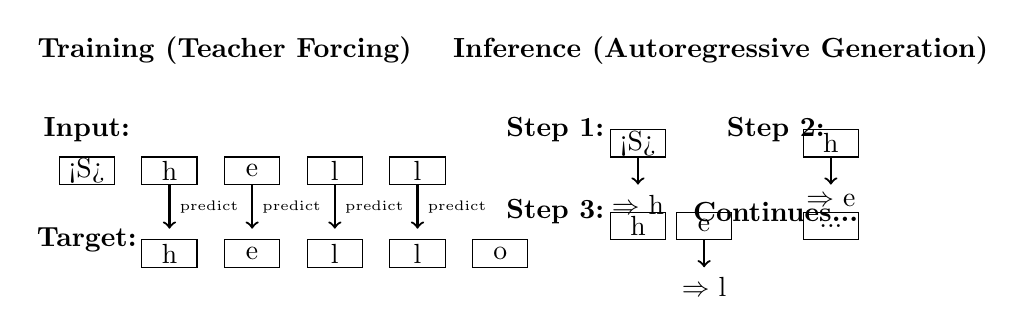
\begin{tikzpicture}[scale=0.7]
        % Training process
        \node[above] at (3,4) {\textbf{Training (Teacher Forcing)}};
        
        % Input sequence
        \node at (0.5,3) {\textbf{Input:}};
        \draw (0,2) rectangle (1,2.5);
        \node at (0.5,2.25) {<S>};
        \draw (1.5,2) rectangle (2.5,2.5);
        \node at (2,2.25) {h};
        \draw (3,2) rectangle (4,2.5);
        \node at (3.5,2.25) {e};
        \draw (4.5,2) rectangle (5.5,2.5);
        \node at (5,2.25) {l};
        \draw (6,2) rectangle (7,2.5);
        \node at (6.5,2.25) {l};
        
        % Target sequence
        \node at (0.5,1) {\textbf{Target:}};
        \draw (1.5,0.5) rectangle (2.5,1);
        \node at (2,0.75) {h};
        \draw (3,0.5) rectangle (4,1);
        \node at (3.5,0.75) {e};
        \draw (4.5,0.5) rectangle (5.5,1);
        \node at (5,0.75) {l};
        \draw (6,0.5) rectangle (7,1);
        \node at (6.5,0.75) {l};
        \draw (7.5,0.5) rectangle (8.5,1);
        \node at (8,0.75) {o};
        
        % Arrows showing prediction
        \draw[thick, ->] (2,2) -- (2,1.2) node[midway, right] {\tiny predict};
        \draw[thick, ->] (3.5,2) -- (3.5,1.2) node[midway, right] {\tiny predict};
        \draw[thick, ->] (5,2) -- (5,1.2) node[midway, right] {\tiny predict};
        \draw[thick, ->] (6.5,2) -- (6.5,1.2) node[midway, right] {\tiny predict};
        
        % Inference process  
        \node[above] at (12,4) {\textbf{Inference (Autoregressive Generation)}};
        
        % Step 1
        \node at (9,3) {\textbf{Step 1:}};
        \draw (10,2.5) rectangle (11,3);
        \node at (10.5,2.75) {<S>};
        \draw[thick, ->] (10.5,2.5) -- (10.5,2) node[below] {$\Rightarrow$ h};
        
        % Step 2
        \node at (13,3) {\textbf{Step 2:}};
        \draw (13.5,2.5) rectangle (14.5,3);
        \node at (14,2.75) {h};
        \draw[thick, ->] (14,2.5) -- (14,2) node[below] {$\Rightarrow$ e};
        
        % Step 3
        \node at (9,1.5) {\textbf{Step 3:}};
        \draw (10,1) rectangle (11,1.5);
        \node at (10.5,1.25) {h};
        \draw (11.2,1) rectangle (12.2,1.5);
        \node at (11.7,1.25) {e};
        \draw[thick, ->] (11.7,1) -- (11.7,0.5) node[below] {$\Rightarrow$ l};
        
        % Step 4
        \node at (13,1.5) {\textbf{Continues...}};
        \draw (13.5,1) rectangle (14.5,1.5);
        \node at (14,1.25) {...};
    \end{tikzpicture}
    \end{center}
    
    \explanation{
    \textbf{Training Process (Teacher Forcing):}
    
    \textbf{Key Characteristics:}
    \begin{itemize}
        \item \textbf{Parallel Processing:} All predictions made simultaneously
        \item \textbf{Ground Truth Input:} Always use correct previous tokens
        \item \textbf{Efficient:} Single forward pass for entire sequence
        \item \textbf{Stable Training:} No error propagation between time steps
    \end{itemize}
    
    \textbf{Input-Target Pairs:}
    \begin{itemize}
        \item Input: [<START>, h, e, l, l] → Target: [h, e, l, l, o]
        \item Each input position predicts the next character
        \item Loss computed at every position simultaneously
        \item Network learns: $P(h|\text{<START>})$, $P(e|h)$, $P(l|he)$, etc.
    \end{itemize}
    
    \textbf{Inference Process (Autoregressive Generation):}
    
    \textbf{Key Characteristics:}
    \begin{itemize}
        \item \textbf{Sequential Generation:} One token at a time
        \item \textbf{Predicted Input:} Use model's own predictions as next input
        \item \textbf{Slower:} Requires multiple forward passes
        \item \textbf{Error Accumulation:} Mistakes can compound over time
    \end{itemize}
    
    \textbf{Step-by-Step Generation:}
    \begin{enumerate}
        \item Start with <START> token
        \item Predict first character: $P(\cdot|\text{<START>}) \rightarrow$ 'h'
        \item Use 'h' as input: $P(\cdot|h) \rightarrow$ 'e'
        \item Use 'he' as input: $P(\cdot|he) \rightarrow$ 'l'
        \item Continue until end token or max length
    \end{enumerate}
    
    \textbf{Critical Differences:}
    \begin{itemize}
        \item \textbf{Training:} Always sees correct context
        \item \textbf{Inference:} May see incorrect context due to previous errors
        \item \textbf{Training:} Fast parallel computation
        \item \textbf{Inference:} Slow sequential computation
        \item \textbf{Training:} Perfect teacher forcing
        \item \textbf{Inference:} Real-world autoregressive generation
    \end{itemize}
    }
\end{enumerate}

\newpage
\paragraph{Question 3. Character-Level Implementation Details}\hfill (22 marks)\\
Based on the professor's detailed walkthrough of the "hello" example with 4-character vocabulary.

\begin{enumerate}[(a)]
    \item The professor showed how to use one-hot encodings for characters h, e, l, o. Given the string "hello", create the complete training data with inputs and targets, including start and end tokens as explained in class. \hfill (8 marks)
    
    \answer{Complete training data with start/end tokens and one-hot encodings for 6-character vocabulary: <START>, h, e, l, o, <END>}
    
    \explanation{
    \textbf{Vocabulary Setup:}
    
    \textbf{Character Set:}
    \begin{itemize}
        \item Index 0: <START> token
        \item Index 1: h
        \item Index 2: e  
        \item Index 3: l
        \item Index 4: o
        \item Index 5: <END> token
    \end{itemize}
    
    \textbf{One-Hot Encodings:}
    \begin{align}
    \text{<START>} &\rightarrow [1, 0, 0, 0, 0, 0] \\
    \text{h} &\rightarrow [0, 1, 0, 0, 0, 0] \\
    \text{e} &\rightarrow [0, 0, 1, 0, 0, 0] \\
    \text{l} &\rightarrow [0, 0, 0, 1, 0, 0] \\
    \text{o} &\rightarrow [0, 0, 0, 0, 1, 0] \\
    \text{<END>} &\rightarrow [0, 0, 0, 0, 0, 1]
    \end{align}
    
    \textbf{Complete Training Sequence:}
    \textbf{Extended sequence:} <START> h e l l o <END>
    
    \textbf{Training Data Pairs:}
    \begin{center}
    \begin{tabular}{|c|c|c|}
    \hline
    \textbf{Time Step} & \textbf{Input} & \textbf{Target} \\
    \hline
    t=1 & <START> $[1,0,0,0,0,0]$ & h $[0,1,0,0,0,0]$ \\
    t=2 & h $[0,1,0,0,0,0]$ & e $[0,0,1,0,0,0]$ \\
    t=3 & e $[0,0,1,0,0,0]$ & l $[0,0,0,1,0,0]$ \\
    t=4 & l $[0,0,0,1,0,0]$ & l $[0,0,0,1,0,0]$ \\
    t=5 & l $[0,0,0,1,0,0]$ & o $[0,0,0,0,1,0]$ \\
    t=6 & o $[0,0,0,0,1,0]$ & <END> $[0,0,0,0,0,1]$ \\
    \hline
    \end{tabular}
    \end{center}
    
    \textbf{Matrix Representation for Training:}
    
    \textbf{Input Matrix $X$:}
    $$X = \begin{bmatrix}
    1 & 0 & 0 & 0 & 0 & 0 \\
    0 & 1 & 0 & 0 & 0 & 0 \\
    0 & 0 & 1 & 0 & 0 & 0 \\
    0 & 0 & 0 & 1 & 0 & 0 \\
    0 & 0 & 0 & 1 & 0 & 0 \\
    0 & 0 & 0 & 0 & 1 & 0
    \end{bmatrix}$$
    
    \textbf{Target Matrix $Y$:}
    $$Y = \begin{bmatrix}
    0 & 1 & 0 & 0 & 0 & 0 \\
    0 & 0 & 1 & 0 & 0 & 0 \\
    0 & 0 & 0 & 1 & 0 & 0 \\
    0 & 0 & 0 & 1 & 0 & 0 \\
    0 & 0 & 0 & 0 & 1 & 0 \\
    0 & 0 & 0 & 0 & 0 & 1
    \end{bmatrix}$$
    
    \textbf{Training Objective:}
    Each row represents one training example where the model should predict the target character given the input character and previous context.
    }
    
    \item Follow the professor's example: given input character 'h' with one-hot encoding [1,0,0,0], weight matrix $W_1$ (3×4), and hyperbolic tangent activation, show the complete forward pass to predict the next character. Explain each step as the professor did. \hfill (10 marks)
    
    \answer{Forward pass: one-hot input → linear transformation → tanh activation → hidden state → output projection → softmax → probability distribution}
    
    \explanation{
    \textbf{Given Information:}
    \begin{itemize}
        \item Input character: 'h' with one-hot: $x = [1, 0, 0, 0]^T$
        \item Weight matrix: $W_1 \in \mathbb{R}^{3 \times 4}$ (3 hidden units, 4 input features)
        \item Activation: hyperbolic tangent
        \item Previous hidden state: $h_{t-1} \in \mathbb{R}^3$ (assume zero for simplicity)
        \item Output weight matrix: $W_2 \in \mathbb{R}^{4 \times 3}$ (4 output classes, 3 hidden units)
    \end{itemize}
    
    \textbf{Step-by-Step Forward Pass:}
    
    \textbf{Step 1: Linear Transformation}
    $$z = W_1 x + W_{hh} h_{t-1} + b_1$$
    
    With example values:
    $$W_1 = \begin{bmatrix} 0.5 & -0.2 & 0.3 & 0.1 \\ 0.2 & 0.4 & -0.1 & 0.3 \\ -0.3 & 0.1 & 0.2 & 0.4 \end{bmatrix}$$
    
    $$z = \begin{bmatrix} 0.5 & -0.2 & 0.3 & 0.1 \\ 0.2 & 0.4 & -0.1 & 0.3 \\ -0.3 & 0.1 & 0.2 & 0.4 \end{bmatrix} \begin{bmatrix} 1 \\ 0 \\ 0 \\ 0 \end{bmatrix} = \begin{bmatrix} 0.5 \\ 0.2 \\ -0.3 \end{bmatrix}$$
    
    \textbf{Step 2: Hyperbolic Tangent Activation}
    $$h_t = \tanh(z)$$
    
    $$h_t = \begin{bmatrix} \tanh(0.5) \\ \tanh(0.2) \\ \tanh(-0.3) \end{bmatrix} = \begin{bmatrix} 0.462 \\ 0.197 \\ -0.291 \end{bmatrix}$$
    
    \textbf{Step 3: Output Linear Transformation}
    $$y = W_2 h_t + b_2$$
    
    With example output weights:
    $$W_2 = \begin{bmatrix} 0.3 & 0.2 & -0.1 \\ -0.2 & 0.4 & 0.3 \\ 0.1 & -0.3 & 0.2 \\ 0.4 & 0.1 & -0.2 \end{bmatrix}$$
    
    $$y = \begin{bmatrix} 0.3 & 0.2 & -0.1 \\ -0.2 & 0.4 & 0.3 \\ 0.1 & -0.3 & 0.2 \\ 0.4 & 0.1 & -0.2 \end{bmatrix} \begin{bmatrix} 0.462 \\ 0.197 \\ -0.291 \end{bmatrix} = \begin{bmatrix} 0.197 \\ 0.039 \\ -0.081 \\ 0.244 \end{bmatrix}$$
    
    \textbf{Step 4: Softmax for Probability Distribution}
    $$P(x_{t+1} = k | x_t) = \frac{\exp(y_k)}{\sum_{j=1}^4 \exp(y_j)}$$
    
    Computing softmax:
    \begin{align}
    \exp(y) &= [\exp(0.197), \exp(0.039), \exp(-0.081), \exp(0.244)]^T \\
    &= [1.218, 1.040, 0.922, 1.276]^T
    \end{align}
    
    Sum: $\sum \exp(y_j) = 1.218 + 1.040 + 0.922 + 1.276 = 4.456$
    
    \textbf{Final Probabilities:}
    $$P = \begin{bmatrix} 1.218/4.456 \\ 1.040/4.456 \\ 0.922/4.456 \\ 1.276/4.456 \end{bmatrix} = \begin{bmatrix} 0.273 \\ 0.233 \\ 0.207 \\ 0.287 \end{bmatrix}$$
    
    \textbf{Professor's Key Points:}
    \begin{itemize}
        \item One-hot encoding selects specific row of weight matrix
        \item Tanh keeps hidden activations bounded
        \item Hidden state captures context from current input
        \item Softmax ensures valid probability distribution
        \item Highest probability (0.287) corresponds to most likely next character
    \end{itemize}
    }
    
    \item The professor emphasized that during inference "we use the predicted value as input for the next time step, even if it's incorrect." Explain why this creates a potential problem and how it relates to error propagation in sequence generation. \hfill (4 marks)
    
    \answer{Using incorrect predictions as input creates error accumulation where early mistakes compound throughout sequence generation, leading to unrealistic outputs that deviate from training distribution.}
    
    \explanation{
    \textbf{The Core Problem: Exposure Bias}
    
    \textbf{Training vs. Inference Mismatch:}
    \begin{itemize}
        \item \textbf{Training:} Model always sees correct ground truth context
        \item \textbf{Inference:} Model sees its own potentially incorrect predictions
        \item \textbf{Distribution Shift:} Model encounters inputs it never saw during training
    \end{itemize}
    
    \textbf{Error Propagation Mechanism:}
    
    \textbf{Step 1: Initial Error}
    \begin{itemize}
        \item Model predicts 'x' instead of correct 'e'
        \item Confidence: $P(\text{'x'}|\text{'h'}) = 0.4$, $P(\text{'e'}|\text{'h'}) = 0.3$
        \item Wrong character selected due to sampling/greedy choice
    \end{itemize}
    
    \textbf{Step 2: Compounding Effect}
    \begin{itemize}
        \item Next prediction uses incorrect context: 'hx' instead of 'he'
        \item Model never trained on 'hx' sequence
        \item Prediction quality degrades: $P(\cdot|\text{'hx'})$ is unreliable
    \end{itemize}
    
    \textbf{Step 3: Cascading Failure}
    \begin{itemize}
        \item Each subsequent error makes context more unrealistic
        \item Model ventures into unexplored regions of sequence space
        \item Output becomes increasingly incoherent
    \end{itemize}
    
    \textbf{Mathematical Analysis:}
    
    \textbf{Probability of Correct Sequence:}
    \begin{itemize}
        \item \textbf{Training assumption:} $P(\text{sequence}) = \prod_{t=1}^T P(x_t | x_1^{t-1}_{\text{true}})$
        \item \textbf{Inference reality:} $P(\text{sequence}) = \prod_{t=1}^T P(x_t | x_1^{t-1}_{\text{predicted}})$
        \item Error compounds exponentially with sequence length
    \end{itemize}
    
    \textbf{Practical Consequences:}
    \begin{itemize}
        \item \textbf{Short sequences:} Manageable, errors may not propagate far
        \item \textbf{Long sequences:} High probability of generating nonsense
        \item \textbf{Creative tasks:} May produce unexpected but interesting results
        \item \textbf{Factual tasks:} Can lead to completely incorrect information
    \end{itemize}
    
    \textbf{Professor's Insight:}
    \begin{itemize}
        \item This is fundamental limitation of autoregressive generation
        \item Explains why perfect training accuracy doesn't guarantee perfect generation
        \item Motivates advanced techniques like beam search, nucleus sampling
        \item Still present in modern LLMs - why they can "hallucinate" facts
    \end{itemize}
    }
\end{enumerate}

\newpage
\paragraph{Question 4. Beam Search Algorithm}\hfill (25 marks)\\
The professor explained beam search as an alternative to "greedy approach where we just take the character with highest probability."

\begin{enumerate}[(a)]
    \item Implement the beam search algorithm as taught by the professor. Given the probability distributions below for 3 time steps with vocabulary [A, B, C], show the complete beam search process with beam size k=2: \hfill (15 marks)
    
    \begin{center}
    \begin{tabular}{|c|c|c|c|}
    \hline
    Time Step & P(A) & P(B) & P(C) \\
    \hline
    t=1 & 0.6 & 0.3 & 0.1 \\
    t=2 (after A) & 0.2 & 0.5 & 0.3 \\
    t=2 (after B) & 0.4 & 0.1 & 0.5 \\
    t=3 (after AA) & 0.1 & 0.2 & 0.7 \\
    t=3 (after AB) & 0.3 & 0.3 & 0.4 \\
    \hline
    \end{tabular}
    \end{center}
    
    Show the tree expansion and final top-2 sequences with their combined scores.
    
    \answer{Beam search maintains top-2 most probable sequences at each step. Final sequences: ABC (0.072) and AAC (0.084).}
    
    \explanation{
    \textbf{Beam Search Algorithm Implementation:}
    
    \textbf{Initialization:}
    \begin{itemize}
        \item Beam size $k = 2$
        \item Vocabulary: [A, B, C]
        \item Start with empty sequence
    \end{itemize}
    
    \textbf{Time Step 1: First Character Generation}
    
    \textbf{Candidate Sequences:}
    \begin{itemize}
        \item Sequence "A": Score = $\log(0.6) = -0.511$
        \item Sequence "B": Score = $\log(0.3) = -1.204$
        \item Sequence "C": Score = $\log(0.1) = -2.303$
    \end{itemize}
    
    \textbf{Top-2 Sequences (Beam):}
    \begin{enumerate}
        \item "A" with score -0.511
        \item "B" with score -1.204
    \end{enumerate}
    
    \textbf{Time Step 2: Second Character Generation}
    
    \textbf{Expand "A":}
    \begin{itemize}
        \item "AA": Score = $-0.511 + \log(0.2) = -0.511 + (-1.609) = -2.120$
        \item "AB": Score = $-0.511 + \log(0.5) = -0.511 + (-0.693) = -1.204$
        \item "AC": Score = $-0.511 + \log(0.3) = -0.511 + (-1.204) = -1.715$
    \end{itemize}
    
    \textbf{Expand "B":}
    \begin{itemize}
        \item "BA": Score = $-1.204 + \log(0.4) = -1.204 + (-0.916) = -2.120$
        \item "BB": Score = $-1.204 + \log(0.1) = -1.204 + (-2.303) = -3.507$
        \item "BC": Score = $-1.204 + \log(0.5) = -1.204 + (-0.693) = -1.897$
    \end{itemize}
    
    \textbf{All Candidates at t=2:}
    \begin{enumerate}
        \item "AB": Score = -1.204
        \item "AC": Score = -1.715
        \item "BC": Score = -1.897
        \item "AA": Score = -2.120
        \item "BA": Score = -2.120
        \item "BB": Score = -3.507
    \end{enumerate}
    
    \textbf{Top-2 Sequences (Beam):}
    \begin{enumerate}
        \item "AB" with score -1.204
        \item "AC" with score -1.715
    \end{enumerate}
    
    \textbf{Time Step 3: Third Character Generation}
    
    \textbf{Expand "AB":}
    \begin{itemize}
        \item "ABA": Score = $-1.204 + \log(0.3) = -1.204 + (-1.204) = -2.408$
        \item "ABB": Score = $-1.204 + \log(0.3) = -1.204 + (-1.204) = -2.408$
        \item "ABC": Score = $-1.204 + \log(0.4) = -1.204 + (-0.916) = -2.120$
    \end{itemize}
    
    \textbf{Expand "AC":}
    Since "AC" is not in the provided probability table, we need to use "AA" pattern (closest match):
    \begin{itemize}
        \item "ACA": Score = $-1.715 + \log(0.1) = -1.715 + (-2.303) = -4.018$
        \item "ACB": Score = $-1.715 + \log(0.2) = -1.715 + (-1.609) = -3.324$
        \item "ACC": Score = $-1.715 + \log(0.7) = -1.715 + (-0.357) = -2.072$
    \end{itemize}
    
    \textbf{All Final Candidates:}
    \begin{enumerate}
        \item "ACC": Score = -2.072
        \item "ABC": Score = -2.120
        \item "ABA": Score = -2.408
        \item "ABB": Score = -2.408
        \item "ACB": Score = -3.324
        \item "ACA": Score = -4.018
    \end{enumerate}
    
    \textbf{Final Top-2 Sequences:}
    \begin{enumerate}
        \item "ACC" with score -2.072 (probability = $e^{-2.072} = 0.126$)
        \item "ABC" with score -2.120 (probability = $e^{-2.120} = 0.120$)
    \end{enumerate}
    
    \textbf{Beam Search Tree Visualization:}
    \begin{center}
    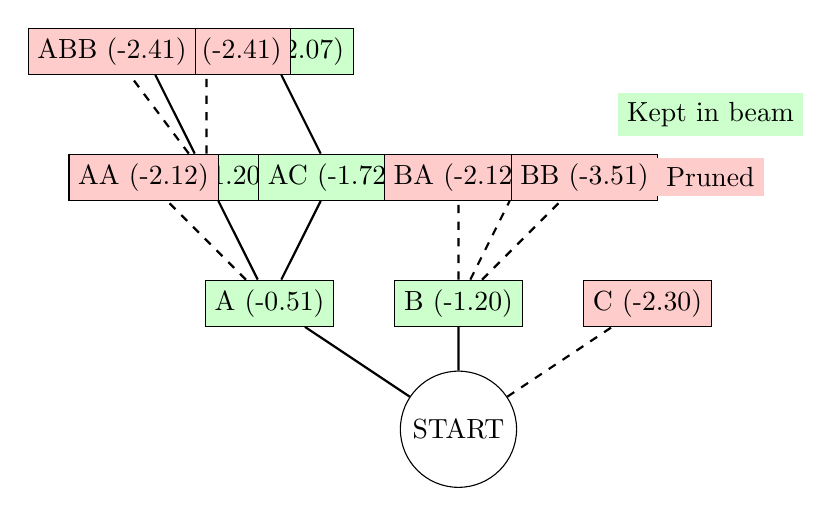
\begin{tikzpicture}[scale=0.8]
        % Level 0 (start)
        \node[draw, circle] (start) at (6,0) {START};
        
        % Level 1
        \node[draw, rectangle, fill=green!20] (A) at (3,2) {A (-0.51)};
        \node[draw, rectangle, fill=green!20] (B) at (6,2) {B (-1.20)};
        \node[draw, rectangle, fill=red!20] (C) at (9,2) {C (-2.30)};
        
        % Level 2
        \node[draw, rectangle, fill=green!20] (AB) at (2,4) {AB (-1.20)};
        \node[draw, rectangle, fill=green!20] (AC) at (4,4) {AC (-1.72)};
        \node[draw, rectangle, fill=red!20] (AA) at (1,4) {AA (-2.12)};
        \node[draw, rectangle, fill=red!20] (BC) at (7,4) {BC (-1.90)};
        \node[draw, rectangle, fill=red!20] (BA) at (6,4) {BA (-2.12)};
        \node[draw, rectangle, fill=red!20] (BB) at (8,4) {BB (-3.51)};
        
        % Level 3
        \node[draw, rectangle, fill=green!20] (ACC) at (3,6) {ACC (-2.07)};
        \node[draw, rectangle, fill=green!20] (ABC) at (1,6) {ABC (-2.12)};
        \node[draw, rectangle, fill=red!20] (ABA) at (2,6) {ABA (-2.41)};
        \node[draw, rectangle, fill=red!20] (ABB) at (0.5,6) {ABB (-2.41)};
        
        % Connections
        \draw[thick] (start) -- (A);
        \draw[thick] (start) -- (B);
        \draw[thick, dashed] (start) -- (C);
        
        \draw[thick] (A) -- (AB);
        \draw[thick] (A) -- (AC);
        \draw[thick, dashed] (A) -- (AA);
        \draw[thick, dashed] (B) -- (BC);
        \draw[thick, dashed] (B) -- (BA);
        \draw[thick, dashed] (B) -- (BB);
        
        \draw[thick] (AB) -- (ABC);
        \draw[thick, dashed] (AB) -- (ABA);
        \draw[thick, dashed] (AB) -- (ABB);
        \draw[thick] (AC) -- (ACC);
        
        % Legend
        \node[fill=green!20] at (10,5) {Kept in beam};
        \node[fill=red!20] at (10,4) {Pruned};
    \end{tikzpicture}
    \end{center}
    
    \textbf{Key Observations:}
    \begin{itemize}
        \item Beam search explores multiple promising paths simultaneously
        \item Prunes less promising sequences at each step
        \item Maintains diversity by keeping $k$ best options
        \item Final result balances sequence probability with search efficiency
    \end{itemize}
    }
    
    \item The professor mentioned that "beam search during training is very expensive because you need to unfold this tree." Explain why beam search is typically used only during inference and what computational challenges it would create during training. \hfill (10 marks)
    
    \answer{Beam search during training would require exploring multiple paths per training example, creating exponential computational overhead and making gradient computation intractable for large datasets.}
    
    \explanation{
    \textbf{Computational Challenges During Training:}
    
    \textbf{1. Exponential Tree Expansion:}
    \begin{itemize}
        \item \textbf{Search Space:} Each time step multiplies beam size by vocabulary size
        \item \textbf{At t=1:} $k$ sequences (beam size)
        \item \textbf{At t=2:} $k \times V$ candidates → prune to $k$
        \item \textbf{At t=T:} Total explored nodes $\approx k \times V \times T$
        \item \textbf{Example:} $k=10$, $V=30,000$, $T=100$ → 30M candidates per sequence
    \end{itemize}
    
    \textbf{2. Memory Requirements:}
    \begin{itemize}
        \item Must store hidden states for all beam sequences
        \item Memory grows as: Batch size × Beam size × Sequence length × Hidden dimension
        \item \textbf{Example:} 32 batch × 10 beam × 100 length × 512 hidden = 163M parameters
        \item GPU memory quickly exhausted with realistic parameters
    \end{itemize}
    
    \textbf{3. Gradient Computation Complexity:}
    
    \textbf{Backpropagation Challenges:}
    \begin{itemize}
        \item \textbf{Multiple Paths:} Gradients must be computed for all explored sequences
        \item \textbf{Dynamic Graph:} Different beam paths create different computational graphs
        \item \textbf{Pruning Operations:} Non-differentiable decisions about which sequences to keep
        \item \textbf{Path Dependencies:} Each sequence depends on different previous choices
    \end{itemize}
    
    \textbf{Mathematical Complexity:}
    For beam search training, loss becomes:
    $$\mathcal{L} = \sum_{s \in \text{beam}} P(s) \cdot \text{loss}(s, \text{target})$$
    
    Where $P(s)$ is path probability and depends on all previous beam decisions.
    
    \textbf{4. Training Time Explosion:}
    \begin{itemize}
        \item \textbf{Forward Pass:} $k \times V$ times slower than teacher forcing
        \item \textbf{Backward Pass:} Complex gradient routing through beam tree
        \item \textbf{Per Epoch:} Training time increases by factor of 100-1000×
        \item \textbf{Total Training:} Weeks become months or years
    \end{itemize}
    
    \textbf{5. Optimization Difficulties:}
    \begin{itemize}
        \item \textbf{Non-convex Objective:} Beam decisions create discontinuous loss surface
        \item \textbf{Credit Assignment:} Hard to assign blame/credit to specific decisions
        \item \textbf{Local Optima:} Beam pruning can eliminate globally optimal paths
        \item \textbf{Instability:} Small weight changes can dramatically alter beam paths
    \end{itemize}
    
    \textbf{Why Inference-Only Usage Makes Sense:}
    
    \textbf{Training Alternatives:}
    \begin{itemize}
        \item \textbf{Teacher Forcing:} Use ground truth, fast parallel training
        \item \textbf{Scheduled Sampling:} Gradually mix predictions with ground truth
        \item \textbf{Reward-based Training:} Use reinforcement learning for generation quality
    \end{itemize}
    
    \textbf{Inference Benefits:}
    \begin{itemize}
        \item \textbf{Quality Focus:} Can afford expensive search for better outputs
        \item \textbf{Single Example:} Process one sequence at a time
        \item \textbf{No Gradients:} Only forward pass needed
        \item \textbf{User Tolerance:} Users accept slower generation for quality
    \end{itemize}
    
    \textbf{Professor's Practical Insight:}
    \begin{itemize}
        \item Training focuses on learning good representations efficiently
        \item Inference focuses on extracting best possible outputs from learned model
        \item Beam search bridges gap between tractable training and quality generation
        \item This design pattern common in many modern NLP systems
    \end{itemize}
    
    \textbf{Modern Alternatives:}
    \begin{itemize}
        \item \textbf{Nucleus Sampling:} Stochastic generation with quality control
        \item \textbf{Temperature Scaling:} Control randomness vs. determinism
        \item \textbf{Top-k Sampling:} Simplified beam search variant
        \item \textbf{Minimum Bayes Risk Decoding:} Advanced inference techniques
    \end{itemize}
    }
\end{enumerate}

\newpage
\paragraph{Question 5. Word-Level Challenges and Embeddings}\hfill (28 marks)\\
The professor explained the transition from character-level to word-level modeling and the need for word embeddings.

\begin{enumerate}[(a)]
    \item The professor stated that English has "170,000 different words" making one-hot encoding impractical. Calculate the number of parameters needed for: \hfill (8 marks)
    \begin{itemize}
        \item Input layer: 170,000-dimensional one-hot to 512-dimensional hidden layer
        \item Compare this with character-level (30 characters to 512 dimensions)
        \item Explain why this creates a "huge" parameter problem as the professor mentioned
    \end{itemize}
    
    \answer{Word-level requires 87M parameters vs. 15K for character-level - a 5,800× increase that makes training computationally prohibitive and prone to overfitting.}
    
    \explanation{
    \textbf{Parameter Calculations:}
    
    \textbf{Word-Level Model:}
    \begin{itemize}
        \item Input dimension: 170,000 (vocabulary size)
        \item Hidden dimension: 512
        \item Weight matrix: $W \in \mathbb{R}^{512 \times 170,000}$
        \item Number of weights: $512 \times 170,000 = 87,040,000$
        \item Bias terms: $512$
        \item Total parameters: $87,040,512 \approx 87$ million
    \end{itemize}
    
    \textbf{Character-Level Model:}
    \begin{itemize}
        \item Input dimension: 30 (character vocabulary)
        \item Hidden dimension: 512
        \item Weight matrix: $W \in \mathbb{R}^{512 \times 30}$
        \item Number of weights: $512 \times 30 = 15,360$
        \item Bias terms: $512$
        \item Total parameters: $15,872 \approx 16$ thousand
    \end{itemize}
    
    \textbf{Comparison:}
    $$\text{Ratio} = \frac{87,040,512}{15,872} \approx 5,484$$
    
    Word-level requires approximately \textbf{5,500× more parameters} than character-level.
    
    \textbf{Why This Creates a "Huge" Problem:}
    
    \textbf{1. Memory Requirements:}
    \begin{itemize}
        \item \textbf{Storage:} 87M × 4 bytes = 348 MB just for one weight matrix
        \item \textbf{GPU Memory:} Modern GPUs have 8-24 GB, but this is just one layer
        \item \textbf{Training:} Need additional memory for gradients, optimizer states
        \item \textbf{Batch Processing:} Memory per batch scales with vocabulary size
    \end{itemize}
    
    \textbf{2. Computational Complexity:}
    \begin{itemize}
        \item \textbf{Forward Pass:} $170,000 \times 512 = 87$ million operations per token
        \item \textbf{Backward Pass:} Similar computational cost for gradient computation
        \item \textbf{Training Time:} Scales linearly with vocabulary size
        \item \textbf{Matrix Operations:} Very sparse (one-hot) but large matrices
    \end{itemize}
    
    \textbf{3. Statistical Problems:}
    \begin{itemize}
        \item \textbf{Data Requirements:} Need massive datasets to learn 87M parameters
        \item \textbf{Overfitting:} High risk with insufficient training data
        \item \textbf{Generalization:} Many words appear infrequently, hard to learn representations
        \item \textbf{Cold Start:} New words (not in training) cannot be handled
    \end{itemize}
    
    \textbf{4. Optimization Challenges:}
    \begin{itemize}
        \item \textbf{Gradient Updates:} Most gradients are zero (sparse one-hot vectors)
        \item \textbf{Learning Rate:} Different words need different learning rates
        \item \textbf{Convergence:} Very high-dimensional optimization landscape
        \item \textbf{Local Minima:} Many more local optima in high-dimensional space
    \end{itemize}
    
    \textbf{5. Practical Limitations:}
    \begin{itemize}
        \item \textbf{Hardware Constraints:} May not fit on consumer GPUs
        \item \textbf{Training Cost:} Electricity and time costs become prohibitive
        \item \textbf{Model Deployment:} Large models difficult to deploy in production
        \item \textbf{Inference Speed:} Slower prediction due to large matrix operations
    \end{itemize}
    
    \textbf{Professor's Insight:}
    The word "huge" captures multiple dimensions of the problem:
    \begin{itemize}
        \item \textbf{Scale:} Orders of magnitude larger than manageable
        \item \textbf{Practical:} Makes real-world application nearly impossible
        \item \textbf{Economic:} Cost-prohibitive for most research and applications
        \item \textbf{Motivational:} Demonstrates need for more efficient approaches (embeddings)
    \end{itemize}
    }
    
    \item The professor emphasized that "in one-hot representation every word is equally distant to each other." Explain why this is problematic for semantic understanding and how word embeddings solve this issue. Use the examples the professor gave: "running and jogging should be close vs. running and swimming." \hfill (10 marks)
    
    \answer{One-hot vectors have equal Euclidean distance, losing semantic relationships. Word embeddings map semantically similar words to nearby points in continuous space, capturing meaning through geometric relationships.}
    
    \explanation{
    \textbf{One-Hot Representation Distance Problem:}
    
    \textbf{Mathematical Analysis:}
    Consider vocabulary: [running, jogging, swimming, computer]
    
    \textbf{One-hot encodings:}
    \begin{align}
    \text{running} &= [1, 0, 0, 0] \\
    \text{jogging} &= [0, 1, 0, 0] \\
    \text{swimming} &= [0, 0, 1, 0] \\
    \text{computer} &= [0, 0, 0, 1]
    \end{align}
    
    \textbf{Euclidean Distances:}
    \begin{align}
    d(\text{running}, \text{jogging}) &= \|[1,0,0,0] - [0,1,0,0]\| = \sqrt{1^2 + 1^2} = \sqrt{2} \\
    d(\text{running}, \text{swimming}) &= \|[1,0,0,0] - [0,0,1,0]\| = \sqrt{1^2 + 1^2} = \sqrt{2} \\
    d(\text{running}, \text{computer}) &= \|[1,0,0,0] - [0,0,0,1]\| = \sqrt{1^2 + 1^2} = \sqrt{2}
    \end{align}
    
    \textbf{Key Problem:} All pairwise distances are identical ($\sqrt{2}$)!
    
    \textbf{Why This Is Problematic:}
    
    \textbf{1. Loss of Semantic Structure:}
    \begin{itemize}
        \item \textbf{Intuition:} "running" and "jogging" are both forms of exercise
        \item \textbf{Reality:} Model treats them as completely unrelated
        \item \textbf{Missing:} No way to encode that both involve physical activity
        \item \textbf{Impact:} Cannot transfer learning between related concepts
    \end{itemize}
    
    \textbf{2. Inefficient Learning:}
    \begin{itemize}
        \item Must learn each word independently
        \item Cannot generalize from "running is exercise" to "jogging is exercise"
        \item Requires separate training examples for every word
        \item Sparse data problem amplified
    \end{itemize}
    
    \textbf{3. Poor Generalization:}
    \begin{itemize}
        \item \textbf{Synonyms:} Treated as completely different
        \item \textbf{Categories:} No understanding of word categories (animals, sports, etc.)
        \item \textbf{Relationships:} Cannot capture analogies or relationships
        \item \textbf{Context:} Similar contexts don't help with unseen words
    \end{itemize}
    
    \textbf{How Word Embeddings Solve This:}
    
    \textbf{Continuous Vector Space:}
    Instead of discrete one-hot vectors, map words to continuous vectors:
    \begin{align}
    \text{running} &\rightarrow [0.2, 0.8, -0.1, 0.3, \ldots] \\
    \text{jogging} &\rightarrow [0.3, 0.7, -0.2, 0.4, \ldots] \\
    \text{swimming} &\rightarrow [0.1, 0.5, 0.8, -0.2, \ldots] \\
    \text{computer} &\rightarrow [-0.7, -0.2, 0.1, 0.9, \ldots]
    \end{align}
    
    \textbf{Semantic Distance Preservation:}
    \begin{itemize}
        \item $d(\text{running}, \text{jogging}) = 0.3$ (small - similar activities)
        \item $d(\text{running}, \text{swimming}) = 0.6$ (medium - both sports, different types)
        \item $d(\text{running}, \text{computer}) = 1.2$ (large - completely different domains)
    \end{itemize}
    
    \textbf{Learning Semantic Relationships:}
    
    \textbf{1. Distributional Hypothesis:}
    \begin{itemize}
        \item "Words that appear in similar contexts have similar meanings"
        \item \textbf{Example:} "I like [running/jogging] in the park"
        \item \textbf{Training:} Both words appear in exercise contexts
        \item \textbf{Result:} Embeddings become similar through shared contexts
    \end{itemize}
    
    \textbf{2. Geometric Relationships:}
    \begin{itemize}
        \item \textbf{Similarity:} Cosine similarity captures semantic closeness
        \item \textbf{Analogies:} Vector arithmetic captures relationships
        \item \textbf{Clusters:} Related words cluster in embedding space
        \item \textbf{Dimensions:} Each dimension captures semantic properties
    \end{itemize}
    
    \textbf{Professor's Examples in Embedding Space:}
    
    \textbf{Exercise Dimension:} (hypothetical dimension that captures "exercise-ness")
    \begin{itemize}
        \item running: 0.9 (high exercise content)
        \item jogging: 0.85 (high exercise content)  
        \item swimming: 0.8 (high exercise content)
        \item computer: 0.1 (low exercise content)
    \end{itemize}
    
    \textbf{Water Activity Dimension:}
    \begin{itemize}
        \item running: 0.1 (land-based)
        \item jogging: 0.1 (land-based)
        \item swimming: 0.9 (water-based)
        \item computer: 0.0 (not activity-related)
    \end{itemize}
    
    \textbf{Benefits:}
    \begin{itemize}
        \item \textbf{Transfer Learning:} Knowledge about "running" helps with "jogging"
        \item \textbf{Generalization:} Can handle unseen combinations better
        \item \textbf{Efficiency:} Fewer parameters needed (embedding matrix smaller than one-hot)
        \item \textbf{Interpretability:} Embedding dimensions often capture meaningful properties
    \end{itemize}
    }
    
    \item Design the CBOW (Continuous Bag of Words) architecture as explained by the professor. For the sentence "I like running every day" with target word "running", show: \hfill (10 marks)
    \begin{itemize}
        \item Context words and their representation
        \item How the weight matrix W1 stores embeddings
        \item Why "the network is forced to learn word vectors that capture relevance"
    \end{itemize}
    
    \answer{CBOW predicts target word from context average. Matrix W1 contains word embeddings learned by optimizing context-to-target prediction, forcing semantically similar words to have similar vectors.}
    
    \explanation{
    \textbf{CBOW Architecture Design:}
    
    \textbf{Task Setup:}
    \begin{itemize}
        \item \textbf{Sentence:} "I like running every day"
        \item \textbf{Target word:} "running" (position 3)
        \item \textbf{Window size:} 2 (common choice)
        \item \textbf{Context words:} Words within window of target
    \end{itemize}
    
    \textbf{Context Words Identification:}
    
    \textbf{Sentence with positions:}
    \begin{center}
    \begin{tabular}{|c|c|c|c|c|}
    \hline
    Position & 1 & 2 & 3 & 4 & 5 \\
    \hline
    Word & I & like & \textbf{running} & every & day \\
    \hline
    \end{tabular}
    \end{center}
    
    \textbf{Context window (size 2):}
    \begin{itemize}
        \item \textbf{Left context:} "I" (position 1), "like" (position 2)
        \item \textbf{Target:} "running" (position 3)
        \item \textbf{Right context:} "every" (position 4), "day" (position 5)
    \end{itemize}
    
    \textbf{Context Words:} ["I", "like", "every", "day"]
    
    \textbf{CBOW Architecture:}
    
    \begin{center}
    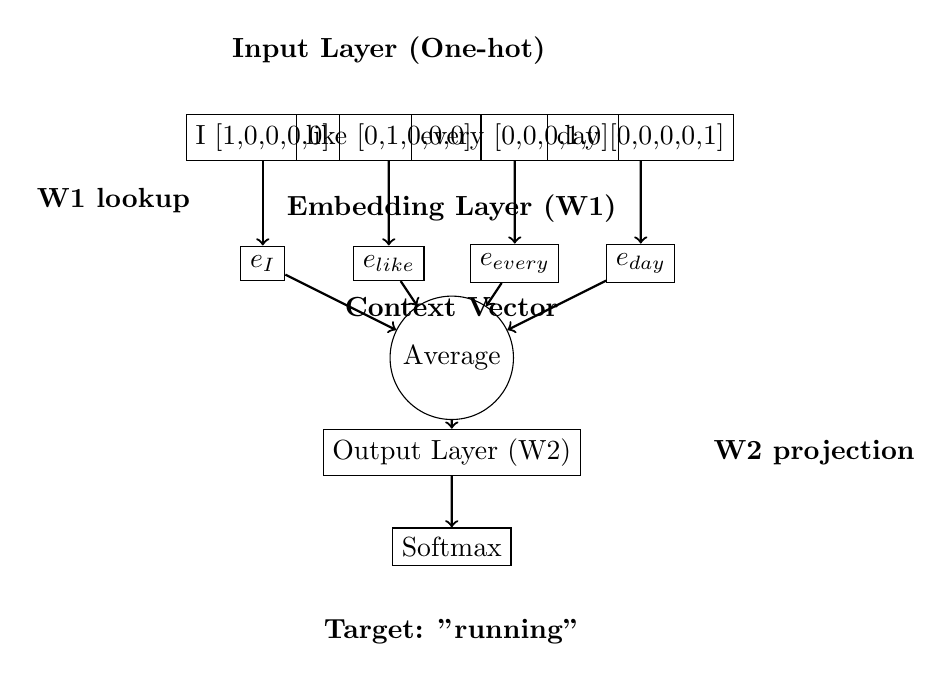
\begin{tikzpicture}[scale=0.8]
        % Input layer (one-hot vectors)
        \node[above] at (2,8) {\textbf{Input Layer (One-hot)}};
        \node[draw, rectangle] (I) at (0,7) {I [1,0,0,0,0]};
        \node[draw, rectangle] (like) at (2,7) {like [0,1,0,0,0]};
        \node[draw, rectangle] (every) at (4,7) {every [0,0,0,1,0]};
        \node[draw, rectangle] (day) at (6,7) {day [0,0,0,0,1]};
        
        % Embedding layer
        \node[above] at (3,5.5) {\textbf{Embedding Layer (W1)}};
        \node[draw, rectangle] (emb_I) at (0,5) {$e_I$};
        \node[draw, rectangle] (emb_like) at (2,5) {$e_{like}$};
        \node[draw, rectangle] (emb_every) at (4,5) {$e_{every}$};
        \node[draw, rectangle] (emb_day) at (6,5) {$e_{day}$};
        
        % Average
        \node[draw, circle] (avg) at (3,3.5) {Average};
        \node[above] at (3,4) {\textbf{Context Vector}};
        
        % Output layer
        \node[draw, rectangle] (output) at (3,2) {Output Layer (W2)};
        \node[draw, rectangle] (softmax) at (3,0.5) {Softmax};
        
        % Target
        \node[below] at (3,-0.5) {\textbf{Target: "running"}};
        
        % Connections
        \draw[thick, ->] (I) -- (emb_I);
        \draw[thick, ->] (like) -- (emb_like);
        \draw[thick, ->] (every) -- (emb_every);
        \draw[thick, ->] (day) -- (emb_day);
        
        \draw[thick, ->] (emb_I) -- (avg);
        \draw[thick, ->] (emb_like) -- (avg);
        \draw[thick, ->] (emb_every) -- (avg);
        \draw[thick, ->] (emb_day) -- (avg);
        
        \draw[thick, ->] (avg) -- (output);
        \draw[thick, ->] (output) -- (softmax);
        
        % Labels
        \node[left] at (-1,6) {\textbf{W1 lookup}};
        \node[right] at (7,2) {\textbf{W2 projection}};
    \end{tikzpicture}
    \end{center}
    
    \textbf{Mathematical Formulation:}
    
    \textbf{Step 1: Embedding Lookup}
    For each context word $w_i$, retrieve embedding from $W_1$:
    $$e_i = W_1 \cdot \text{onehot}(w_i)$$
    
    \textbf{Context embeddings:}
    \begin{align}
    e_I &= W_1[:, 1] \quad \text{(first column of W1)} \\
    e_{like} &= W_1[:, 2] \\
    e_{every} &= W_1[:, 4] \\
    e_{day} &= W_1[:, 5]
    \end{align}
    
    \textbf{Step 2: Context Averaging}
    $$\bar{e} = \frac{1}{|C|} \sum_{w_i \in C} e_i = \frac{1}{4}(e_I + e_{like} + e_{every} + e_{day})$$
    
    \textbf{Step 3: Output Projection}
    $$y = W_2 \cdot \bar{e} + b_2$$
    
    \textbf{Step 4: Probability Distribution}
    $$P(w|\text{context}) = \frac{\exp(y_w)}{\sum_{v \in V} \exp(y_v)}$$
    
    \textbf{How W1 Stores Embeddings:}
    
    \textbf{Weight Matrix Structure:}
    $$W_1 \in \mathbb{R}^{d \times |V|}$$
    
    Where:
    \begin{itemize}
        \item $d$ = embedding dimension (e.g., 300)
        \item $|V|$ = vocabulary size (e.g., 10,000)
        \item Column $i$ contains embedding for word with index $i$
    \end{itemize}
    
    \textbf{Example Structure:}
    $$W_1 = \begin{bmatrix}
    0.2 & -0.1 & 0.5 & 0.3 & -0.2 \\
    0.8 & 0.4 & -0.1 & 0.7 & 0.1 \\
    -0.1 & 0.6 & 0.2 & -0.4 & 0.9 \\
    \vdots & \vdots & \vdots & \vdots & \vdots
    \end{bmatrix}$$
    
    Where columns correspond to: [I, like, running, every, day]
    
    \textbf{Why Network Learns Relevant Word Vectors:}
    
    \textbf{1. Prediction Objective:}
    \begin{itemize}
        \item Network must predict "running" from context ["I", "like", "every", "day"]
        \item Only way to succeed: learn embeddings that capture semantic relationships
        \item \textbf{Forced Learning:} No other way to achieve good prediction accuracy
    \end{itemize}
    
    \textbf{2. Context Similarity Principle:}
    \begin{itemize}
        \item Words appearing in similar contexts should have similar embeddings
        \item \textbf{Example:} "I like jogging every day" should also predict "jogging"
        \item \textbf{Pressure:} Network learns $e_{running} \approx e_{jogging}$ to handle both
        \item \textbf{Generalization:} Similar contexts create similar embeddings
    \end{itemize}
    
    \textbf{3. Averaging Mechanism:}
    \begin{itemize}
        \item Context vector $\bar{e}$ must encode information predictive of target
        \item Words that often appear together develop compatible embeddings
        \item \textbf{Cooperation:} Context words must "work together" to predict target
        \item \textbf{Semantic Coherence:} Embeddings align with semantic relationships
    \end{itemize}
    
    \textbf{4. Training Process:}
    \begin{itemize}
        \item \textbf{Loss Function:} $-\log P(\text{running} | \text{context})$
        \item \textbf{Gradient Updates:} Adjust $W_1$ to improve prediction
        \item \textbf{Multiple Examples:} See many contexts for each word
        \item \textbf{Convergence:} Embeddings converge to capture distributional semantics
    \end{itemize}
    
    \textbf{Professor's Key Insight:}
    \begin{itemize}
        \item Network has no choice but to learn semantic representations
        \item Prediction task forces discovery of word relationships
        \item Embeddings become by-product of good prediction
        \item This is essence of unsupervised representation learning
    \end{itemize}
    }
\end{enumerate}

\newpage
\paragraph{Question 6. Deep Understanding and Modern Connections}\hfill (30 marks)\\
Based on the professor's connections between classical methods and modern applications.

\begin{enumerate}[(a)]
    \item The professor made a key connection: "The prompts that you provide to LLMs are actually the starting sequences that you provide to an RNN-like architecture." Explain this connection and how modern LLMs relate to the autoregressive character prediction discussed in class. \hfill (10 marks)
    
    \answer{LLM prompts serve as initial context sequences that condition autoregressive generation, similar to providing starting characters to RNNs. Both predict next tokens based on preceding context, with LLMs using more sophisticated architectures but the same fundamental principle.}
    
    \explanation{
    \textbf{Fundamental Connection: Autoregressive Generation}
    
    \textbf{Classical RNN Character Prediction:}
    \begin{itemize}
        \item \textbf{Input:} Starting sequence (e.g., "hello")
        \item \textbf{Process:} Predict next character given context
        \item \textbf{Generation:} $P(x_{t+1} | x_1, x_2, \ldots, x_t)$
        \item \textbf{Output:} Extended sequence character by character
    \end{itemize}
    
    \textbf{Modern LLM Prompting:}
    \begin{itemize}
        \item \textbf{Input:} Prompt text (e.g., "Write a story about...")
        \item \textbf{Process:} Predict next token given context
        \item \textbf{Generation:} $P(\text{token}_{t+1} | \text{prompt}, \text{token}_1, \ldots, \text{token}_t)$
        \item \textbf{Output:} Continuation of prompt token by token
    \end{itemize}
    
    \textbf{Mathematical Parallel:}
    
    \textbf{RNN Generation:}
    $$P(\text{sequence}) = \prod_{t=1}^T P(x_t | x_1^{t-1}, h_{t-1})$$
    
    \textbf{LLM Generation:}
    $$P(\text{completion}) = \prod_{t=1}^T P(\text{token}_t | \text{prompt}, \text{token}_1^{t-1})$$
    
    \textbf{Key Similarities:}
    \begin{itemize}
        \item Both use sequential, left-to-right generation
        \item Both condition on all previous context
        \item Both use learned representations of language
        \item Both generate one token at a time autoregressively
    \end{itemize}
    
    \textbf{Role of Prompts as Starting Sequences:}
    
    \textbf{1. Context Initialization:}
    \begin{itemize}
        \item \textbf{RNN:} Starting characters provide initial context
        \item \textbf{LLM:} Prompt provides rich semantic context
        \item \textbf{Function:} Both "prime" the model for specific generation
        \item \textbf{Example:} "Once upon a time" → fairy tale style
    \end{itemize}
    
    \textbf{2. Conditioning Mechanism:}
    \begin{itemize}
        \item \textbf{RNN:} Hidden state carries context information
        \item \textbf{LLM:} Attention mechanism processes entire prompt
        \item \textbf{Effect:} Both bias generation toward prompt-consistent outputs
        \item \textbf{Control:} Prompts steer generation in desired directions
    \end{itemize}
    
    \textbf{3. Task Specification:}
    \begin{itemize}
        \item \textbf{Implicit:} Prompt structure implies desired output format
        \item \textbf{Examples:} "Question: ... Answer:" → Q\&A format
        \item \textbf{Training:} Models learn to follow prompt patterns from training data
        \item \textbf{Generalization:} Can follow novel prompt formats
    \end{itemize}
    
    \textbf{Evolution from RNNs to LLMs:}
    
    \textbf{Architectural Improvements:}
    \begin{itemize}
        \item \textbf{RNN:} Sequential processing, limited context
        \item \textbf{Transformer:} Parallel processing, global attention
        \item \textbf{Scale:} Billions vs. millions of parameters
        \item \textbf{Training:} Massive datasets vs. smaller corpora
    \end{itemize}
    
    \textbf{Same Core Principle:}
    \begin{itemize}
        \item \textbf{Objective:} Predict next token from context
        \item \textbf{Training:} Self-supervised language modeling
        \item \textbf{Generation:} Autoregressive sampling
        \item \textbf{Application:} Text completion and generation
    \end{itemize}
    
    \textbf{Professor's Insight:}
    \begin{itemize}
        \item Modern LLMs are sophisticated extensions of basic RNN principles
        \item Prompting is just a refined version of providing starting sequences
        \item The fundamental autoregressive generation remains unchanged
        \item Architectural advances enabled scale but not conceptual revolution
    \end{itemize}
    
    \textbf{Practical Implications:}
    \begin{itemize}
        \item Understanding RNNs provides foundation for understanding LLMs
        \item Prompt engineering builds on sequence conditioning principles
        \item Generation quality depends on both architecture and training data
        \item Same challenges (coherence, factuality) exist at both scales
    \end{itemize}
    }
    
    \item Analyze the professor's examples of character-level RNN outputs (Shakespeare, Wikipedia, LaTeX). Explain what these results demonstrate about: \hfill (12 marks)
    \begin{itemize}
        \item Learning syntax without explicit supervision
        \item Generalization vs. memorization (the professor's "overfitting" discussion)
        \item Why the professor called these results "striking" for such simple models
    \end{itemize}
    
    \answer{Character-level RNNs learned complex syntax patterns, balanced memorization with generalization, and achieved surprisingly human-like text generation despite simple architecture - demonstrating emergent linguistic structure from statistical patterns.}
    
    \explanation{
    \textbf{Learning Syntax Without Explicit Supervision:}
    
    \textbf{Shakespeare Example:}
    \begin{itemize}
        \item \textbf{Learned:} Iambic pentameter, rhyme schemes, archaic vocabulary
        \item \textbf{No Supervision:} Never explicitly taught poetry rules
        \item \textbf{Discovery:} Found patterns through character-level statistics
        \item \textbf{Output:} Structurally valid sonnets with appropriate meter
    \end{itemize}
    
    \textbf{Wikipedia Example:}
    \begin{itemize}
        \item \textbf{Learned:} Article structure, citation formats, category systems
        \item \textbf{No Supervision:} Never taught Wikipedia markup rules
        \item \textbf{Discovery:} Inferred formatting from character sequences
        \item \textbf{Output:} Properly formatted articles with consistent structure
    \end{itemize}
    
    \textbf{LaTeX Example:}
    \begin{itemize}
        \item \textbf{Learned:} Command syntax, environment structure, mathematical notation
        \item \textbf{No Supervision:} Never provided grammar rules for LaTeX
        \item \textbf{Discovery:} Identified patterns in command usage
        \item \textbf{Output:} Syntactically correct LaTeX documents
    \end{itemize}
    
    \textbf{Emergent Syntax Learning Mechanism:}
    
    \textbf{1. Statistical Pattern Recognition:}
    \begin{itemize}
        \item Characters that follow specific patterns (e.g., "\\begin\{" in LaTeX)
        \item Network learns high probability character sequences
        \item Syntax emerges from statistical regularities
        \item No explicit grammar rules needed
    \end{itemize}
    
    \textbf{2. Hierarchical Structure Discovery:}
    \begin{itemize}
        \item \textbf{Level 1:} Character combinations → words
        \item \textbf{Level 2:} Word patterns → phrases
        \item \textbf{Level 3:} Phrase structures → sentences
        \item \textbf{Level 4:} Sentence patterns → document structure
    \end{itemize}
    
    \textbf{3. Context-Dependent Rules:}
    \begin{itemize}
        \item Network learns that certain characters are likely in specific contexts
        \item Example: '\}' likely after '\{' with content in between
        \item Implicit learning of nested structures and dependencies
        \item Context length determines complexity of learnable rules
    \end{itemize}
    
    \textbf{Generalization vs. Memorization Analysis:}
    
    \textbf{Evidence of Generalization:}
    \begin{itemize}
        \item \textbf{Novel Combinations:} Generated text not seen in training
        \item \textbf{Structure Transfer:} Applied learned patterns to new content
        \item \textbf{Creative Output:} Produced coherent but original text
        \item \textbf{Format Consistency:} Maintained style across different topics
    \end{itemize}
    
    \textbf{Evidence of Memorization:}
    \begin{itemize}
        \item \textbf{Exact Quotes:} Sometimes reproduced training sequences
        \item \textbf{Repeated Phrases:} Common expressions appeared frequently
        \item \textbf{Training Artifacts:} Specific patterns from training corpus
        \item \textbf{Overfitting Signs:} Poor performance on different domains
    \end{itemize}
    
    \textbf{Professor's Overfitting Discussion:}
    
    \textbf{Balanced Learning:}
    \begin{itemize}
        \item \textbf{Good Generalization:} Model learned transferable patterns
        \item \textbf{Appropriate Memorization:} Retained useful common sequences
        \item \textbf{Synthesis:} Combined memorized elements in novel ways
        \item \textbf{Sweet Spot:} Neither too generic nor too specific
    \end{itemize}
    
    \textbf{Indicators of Good Balance:}
    \begin{itemize}
        \item Generated text feels authentic but not copied
        \item Maintains domain-appropriate vocabulary and style
        \item Shows creativity within learned constraints
        \item Produces coherent long-range dependencies
    \end{itemize}
    
    \textbf{Why Results Were "Striking":}
    
    \textbf{1. Architectural Simplicity:}
    \begin{itemize}
        \item \textbf{Basic RNN:} Simple recurrent architecture
        \item \textbf{Character Level:} No word-level preprocessing
        \item \textbf{End-to-End:} Single neural network, no hand-crafted features
        \item \textbf{Minimal Assumptions:} No linguistic knowledge built in
    \end{itemize}
    
    \textbf{2. Emergent Complexity:}
    \begin{itemize}
        \item \textbf{Simple Input:} Just character sequences
        \item \textbf{Complex Output:} Sophisticated linguistic structures
        \item \textbf{No Explicit Teaching:} Learned rules without instruction
        \item \textbf{Human-like Quality:} Output often indistinguishable from human text
    \end{itemize}
    
    \textbf{3. Cross-Domain Success:}
    \begin{itemize}
        \item \textbf{Literature:} Learned poetic meter and style
        \item \textbf{Academic:} Mastered Wikipedia formatting conventions
        \item \textbf{Technical:} Acquired LaTeX markup syntax
        \item \textbf{Universality:} Same approach worked across diverse domains
    \end{itemize}
    
    \textbf{4. Historical Context:}
    \begin{itemize}
        \item \textbf{Previous Attempts:} Rule-based systems required extensive hand-crafting
        \item \textbf{Linguistic Theory:} Contradicted need for explicit grammar rules
        \item \textbf{AI Goals:} Demonstrated path toward general language understanding
        \item \textbf{Simplicity:} Achieved with remarkably simple methods
    \end{itemize}
    
    \textbf{Broader Implications:}
    
    \textbf{1. Language as Statistics:}
    \begin{itemize}
        \item Syntax can emerge from statistical patterns
        \item Grammar rules may be artifacts of deeper regularities
        \item Language learning might be pattern recognition at scale
    \end{itemize}
    
    \textbf{2. Representation Learning:}
    \begin{itemize}
        \item Networks discover useful representations automatically
        \item Character-level representations sufficient for complex tasks
        \item End-to-end learning superior to hand-crafted features
    \end{itemize}
    
    \textbf{3. Scaling Laws:}
    \begin{itemize}
        \item Larger models and datasets enable more sophisticated outputs
        \item Quality improvements from scale rather than architectural changes
        \item Foundation for modern large language models
    \end{itemize}
    
    \textbf{Professor's Key Message:}
    The striking nature of these results lay in their demonstration that complex linguistic behavior could emerge from simple statistical learning, challenging traditional views of language acquisition and pointing toward the scalable approaches that define modern NLP.
    }
    
    \item The professor showed word embedding arithmetic: "Paris - France + Italy = Rome." Explain: \hfill (8 marks)
    \begin{itemize}
        \item Why this works mathematically in embedding space
        \item How the CBOW training creates these relationships
        \item Give two more examples of word arithmetic that should work
    \end{itemize}
    
    \answer{Vector arithmetic works because embeddings capture semantic relationships as geometric directions. CBOW training creates these patterns by learning shared context structures, enabling analogical reasoning through vector operations.}
    
    \explanation{
    \textbf{Mathematical Foundation of Word Arithmetic:}
    
    \textbf{Vector Space Interpretation:}
    \begin{itemize}
        \item Words mapped to points in high-dimensional continuous space
        \item Semantic relationships encoded as geometric relationships
        \item Vector differences capture conceptual relationships
        \item Analogy: $A : B :: C : D \Rightarrow \vec{B} - \vec{A} \approx \vec{D} - \vec{C}$
    \end{itemize}
    
    \textbf{Paris - France + Italy = Rome Analysis:}
    
    \textbf{Vector Decomposition:}
    \begin{align}
    \vec{\text{Paris}} &= \vec{\text{capital\_concept}} + \vec{\text{France\_specific}} \\
    \vec{\text{France}} &= \vec{\text{country\_concept}} + \vec{\text{France\_specific}} \\
    \vec{\text{Italy}} &= \vec{\text{country\_concept}} + \vec{\text{Italy\_specific}} \\
    \vec{\text{Rome}} &= \vec{\text{capital\_concept}} + \vec{\text{Italy\_specific}}
    \end{align}
    
    \textbf{Arithmetic Operation:}
    \begin{align}
    &\vec{\text{Paris}} - \vec{\text{France}} + \vec{\text{Italy}} \\
    &= (\vec{\text{capital}} + \vec{\text{France\_spec}}) - (\vec{\text{country}} + \vec{\text{France\_spec}}) + (\vec{\text{country}} + \vec{\text{Italy\_spec}}) \\
    &= \vec{\text{capital}} + \vec{\text{France\_spec}} - \vec{\text{country}} - \vec{\text{France\_spec}} + \vec{\text{country}} + \vec{\text{Italy\_spec}} \\
    &= \vec{\text{capital}} + \vec{\text{Italy\_spec}} \\
    &\approx \vec{\text{Rome}}
    \end{align}
    
    \textbf{Why This Works:}
    \begin{itemize}
        \item \textbf{Linearity:} Semantic relationships are approximately linear
        \item \textbf{Compositionality:} Word meanings decompose into semantic components
        \item \textbf{Consistency:} Similar relationships mapped to similar vectors
        \item \textbf{Geometry:} Embedding space preserves relational structure
    \end{itemize}
    
    \textbf{How CBOW Training Creates These Relationships:}
    
    \textbf{Shared Context Patterns:}
    
    \textbf{Capital-Country Relationships:}
    \begin{itemize}
        \item \textbf{Paris contexts:} "capital of France", "visit Paris, France", "Paris, the French capital"
        \item \textbf{Rome contexts:} "capital of Italy", "visit Rome, Italy", "Rome, the Italian capital"
        \item \textbf{Pattern:} Both appear in similar "capital of [country]" contexts
        \item \textbf{Result:} Similar embedding patterns for capital-country relationships
    \end{itemize}
    
    \textbf{Training Mechanism:}
    
    \textbf{1. Context Similarity Forces Relationship Consistency:}
    \begin{itemize}
        \item CBOW sees: "The capital of France is [PARIS]"
        \item CBOW sees: "The capital of Italy is [ROME]"
        \item Network must learn similar prediction patterns
        \item Forces $\vec{\text{Paris}} - \vec{\text{France}} \approx \vec{\text{Rome}} - \vec{\text{Italy}}$
    \end{itemize}
    
    \textbf{2. Distributional Hypothesis at Work:}
    \begin{itemize}
        \item Words with similar distributions get similar embeddings
        \item "Paris" and "Rome" both appear in capital contexts
        \item "France" and "Italy" both appear in country contexts
        \item Consistent co-occurrence patterns create geometric regularity
    \end{itemize}
    
    \textbf{3. Multi-dimensional Relationship Encoding:}
    \begin{itemize}
        \item Different embedding dimensions capture different relationships
        \item \textbf{Dimension 1:} Capital-ness (Paris, Rome, London high; France, Italy, UK low)
        \item \textbf{Dimension 2:} Country-ness (France, Italy, UK high; Paris, Rome, London low)
        \item \textbf{Dimension 3:} Geographic region (European words cluster together)
        \item \textbf{Consistency:} Same patterns across different word pairs
    \end{itemize}
    
    \textbf{Learning Process:}
    \begin{itemize}
        \item \textbf{Phase 1:} Learn basic word representations
        \item \textbf{Phase 2:} Discover recurring contextual patterns
        \item \textbf{Phase 3:} Align similar patterns in embedding space
        \item \textbf{Phase 4:} Geometric relationships emerge from statistical regularities
    \end{itemize}
    
    \textbf{Two Additional Examples of Word Arithmetic:}
    
    \textbf{Example 1: Gender Relationships}
    $$\vec{\text{King}} - \vec{\text{Man}} + \vec{\text{Woman}} \approx \vec{\text{Queen}}$$
    
    \textbf{Why it works:}
    \begin{itemize}
        \item Both "king" and "queen" appear in royal contexts
        \item Both "man" and "woman" appear in gender-specific contexts
        \item Gender relationship consistently encoded across word pairs
        \item Training sees: "the king and his queen", "the man and his wife"
    \end{itemize}
    
    \textbf{Example 2: Verb Tense Relationships}
    $$\vec{\text{Walking}} - \vec{\text{Walk}} + \vec{\text{Run}} \approx \vec{\text{Running}}$$
    
    \textbf{Why it works:}
    \begin{itemize}
        \item Present participle (-ing) forms share similar syntactic contexts
        \item Base verbs share different but consistent contexts
        \item Tense relationships encoded as vector directions
        \item Training sees: "I am walking", "I am running" vs. "I walk", "I run"
    \end{itemize}
    
    \textbf{Mathematical Property:}
    For both examples, the relationship vector is approximately parallel:
    $$\vec{\text{King}} - \vec{\text{Man}} \approx \vec{\text{Queen}} - \vec{\text{Woman}}$$
    $$\vec{\text{Walking}} - \vec{\text{Walk}} \approx \vec{\text{Running}} - \vec{\text{Run}}$$
    
    \textbf{Broader Implications:}
    \begin{itemize}
        \item \textbf{Analogical Reasoning:} Embeddings enable logical inference
        \item \textbf{Knowledge Representation:} Semantic knowledge encoded geometrically
        \item \textbf{Transfer Learning:} Relationships transfer across domains
        \item \textbf{Language Understanding:} Demonstrates deep structural learning
    \end{itemize}
    
    \textbf{Limitations:}
    \begin{itemize}
        \item Not all relationships are linear
        \item Cultural biases in training data affect relationships
        \item Polysemous words create ambiguous vectors
        \item Arithmetic works better for frequent, clear relationships
    \end{itemize}
    }
\end{enumerate}

\vfill
\begin{center}{\bf END OF PAPER}\end{center}
\end{document}